\documentclass[nofootinbib,twocolumn,preprintnumbers]{revtex4-1}
%\usepackage[dvips]{graphicx}
\pdfoutput=1
\usepackage{amsmath,amsthm,amssymb,multirow,psfrag}
\usepackage{epsfig}
\usepackage{color}
\usepackage{slashed}
\usepackage{soul}
\graphicspath{{./Figures/}}


\begin{document}

%%%%%%%%%%%new definitions: 
\def\lsim{\mathrel{\rlap{\lower4pt\hbox{\hskip1pt$\sim$}}
  \raise1pt\hbox{$<$}}}
\def\gsim{\mathrel{\rlap{\lower4pt\hbox{\hskip1pt$\sim$}}
  \raise1pt\hbox{$>$}}}
\newcommand{\vev}[1]{ \left\langle {#1} \right\rangle }
\newcommand{\bra}[1]{ \langle {#1} | }
\newcommand{\ket}[1]{ | {#1} \rangle }
\newcommand{\ev}{ {\rm eV} }
\newcommand{\kev}{{\rm keV}}
\newcommand{\mev}{{\rm MeV}}
\newcommand{\gev}{{\mathrm GeV}}
\newcommand{\tev}{{\rm TeV}}
\newcommand{\mpl}{$M_{Pl}$}
\newcommand{\mw}{$M_{W}$}
\newcommand{\Ft}{F_{T}}
\newcommand{\Zparity}{\mathbb{Z}_2}
\newcommand{\BLambda}{\boldsymbol{\lambda}}
\newcommand{\met}{\;\not\!\!\!{E}_T}
\newcommand{\beq}{\begin{equation}}
\newcommand{\eeq}{\end{equation}}
\newcommand{\bea}{\begin{eqnarray}}
\newcommand{\eea}{\end{eqnarray}}
\newcommand{\nn}{\nonumber}
\newcommand{\hc}{\mathrm{h.c.}}
\newcommand{\eps}{\epsilon}
\newcommand{\bwt}{\begin{widetext}}
\newcommand{\ewt}{\end{widetext}}
\newcommand{\draftnote}[1]{{\bf\color{blue} #1}}
\newcommand{\cO}{{\cal O}}
\newcommand{\cL}{{\cal L}}
\newcommand{\cM}{{\cal M}}
%References  
\newcommand{\fref}[1]{Fig.~\ref{fig:#1}} 
\newcommand{\eref}[1]{Eq.~\eqref{eq:#1}} 
\newcommand{\aref}[1]{Appendix~\ref{app:#1}}
\newcommand{\sref}[1]{Section~\ref{sec:#1}}
\newcommand{\tref}[1]{Table~\ref{tab:#1}}
%\title{\LARGE{{\bf{Piled up gravitational waves:} \\
%\bf{Searching for new signals of $N$naturalness} }}}
\title{\LARGE{{\bf{Gravitational Wave Signals from Multiple Hidden Sectors} \\
}}}
\author{{\bf {Paul Archer-Smith, Dylan Linthorne, and Daniel Stolarski}}}
\affiliation{
Ottawa-Carleton  Institute  for  Physics,  Carleton  University,\\
1125  Colonel  By  Drive,  Ottawa,  Ontario  K1S  5B6,  Canada
}
\email{
PaulSmith3@cmail.carleton.ca \\
Dylan.linthorne@carleton.ca \\
stolar@physics.carleton.ca
}
\begin{abstract}
We explore the possibility of detecting gravitational waves generated by 1st order phase transitions in multiple dark sectors. $N$naturalness is taken as a sample model that features multiple additional sectors, many of which undergo phase transitions that produce gravitational waves. We examine the cosmological history of this framework and determine the gravitational wave profiles generated. These profiles are checked against projections of next generation gravitational wave experiments, demonstrating that multiple hidden sectors can indeed produce unique gravitational wave signatures that will be probed by these future experiments. 
\end{abstract}
\maketitle
%%%%%%%%%%%%%%%%%%%%%%%%%%%%%
\section{Introduction} 
\label{sec:intro} 
The recent experimental detection of gravitational waves~\cite{Abbott:2016blz} gives humanity a new way to observe the universe. Future experiments~\cite{Seto:2001qf,Crowder:2005nr,Harry:2006fi,Sathyaprakash:2012jk,Janssen:2014dka,2017arXiv170200786A,Sato:2017dkf} will greatly expand the frequency range observable. Thus far, experiments have only observed recent events such as black hole mergers, but phase transitions in the early universe can leave an imprint as a \textit{stochastic} gravitational wave background~\cite{Witten:1984rs,Hogan:1984hx,Hogan:1986qda,PhysRevLett.65.3080,Caprini:2015zlo,Mazumdar:2018dfl}. Thus, searches for this background of gravitational waves can give direct information of the history of the universe before big bang nucleosynthesis. 
Because gravity is universal, gravitational waves can allow us to probe hidden sectors that couple very weakly, or not at all, to the Standard Model as long they are reheated after inflation. This was first explored in~\cite{Schwaller:2015tja}, and there has been significant work on this idea since~\cite{Jaeckel:2016jlh,Addazi:2016fbj,Hardy:2016mns,Dienes:2016vei,Tsumura:2017knk,Acharya:2017szw,Bernal:2017kxu,Aoki:2017aws,Heikinheimo:2018esa,Geller:2018mwu,Croon:2018erz,Baldes:2018emh,Bai:2018dxf,Breitbach:2018ddu,Fairbairn:2019xog,Helmboldt:2019pan,Caputo:2019wsd,Bertone:2019irm}. 

In this work, we explore the possibility of having multiple decoupled hidden sectors. Large numbers of hidden sectors can solve the hierarchy problem as in the Dvali Redi model~\cite{Dvali:2009ne}, in the more recently explored $N$naturalness~\cite{Arkani-Hamed:2016rle} framework, or in orbifold Higgs models~\cite{Craig:2014aea,Craig:2014roa}. They can also be motivated by dark matter considerations~\cite{Dienes:2011ja,Dienes:2011sa,Dienes:2016vei}. 
Motivated by solutions to the hierachy problem, we consider hidden sectors with the same particle content as the Standard Model that have all dimensionless couplings (defined at some high scale) equal to those of the Standard Model. The only parameter that varies across sectors is the dimension two Higgs mass squared parameter, $m_H^2$. This simple ansatz can lead to very rich phenomenology and interesting gravitational wave spectra, but we stress that it is only a starting point for exploring the space of theories with multiple hidden sectors.
In this setup, there are two qualitatively different kinds of sectors:
\begin{itemize}
\item \textbf{Standard Sectors}: Those with $m_H^2 < 0$ where electroweak symmetry is broken by the vacuum expectation value (VEV) of a fundamental scalar. As in~\cite{Arkani-Hamed:2016rle}, we assume that the standard sector with the smallest absolute value of $m_H^2$ is the Standard Model.
\item \textbf{Exotic Sectors}: Those with  $m_H^2 > 0$. In this case, electroweak symmetry breaking is preserved below the mass of the Higgs, and broken by the confinement of QCD~\cite{Arkani-Hamed:2016rle,Pisarski:1983ms}.
\end{itemize}
Cosmological observations, particularly limits on extra relativistic degrees of freedom at the time of Big Bang Nucleosynthesis and the time of the formation of the cosmic microwave background (CMB)~\cite{Aghanim:2018eyx}, require that most of the energy in the universe is in the Standard Model sector as we will quantify. Therefore, the hidden sectors cannot be in thermal equilibrium at any time, and the physics of reheating must dump energy preferentially in the Standard Model sector. This can be accomplished with primodial axion-like particle (ALP) models~\cite{MARSH20161,PhysRevLett.121.201303} and with the reheaton method~\cite{Arkani-Hamed:2016rle}. We will also explore alternative parameterizations of reheating that satisfy this condition.
In all the above models, there is some energy in the hidden sectors, and these sectors undergo thermal evolution independent of the SM sector. If their initial reheating temperature is above their weak scale, the standard sectors will undergo phase transitions associated with the breaking of electroweak symmetry and with confinement of QCD. The exotic sectors will also undergo a phase transition when QCD confines and electroweak symmetry is broken simultaneously. The condition for these transitions to leave imprints on the stochastic gravitational wave spectrum is that they strongly first order phase transitions (SFOPT)~\cite{Witten:1984rs,Hogan:1984hx,Hogan:1986qda,PhysRevLett.65.3080}. This does not occur at either the electroweak or QCD phase transition in the SM, but as we will show, it does happen in some standard sectors, and in \textit{all} exotic sectors that reheat above the QCD phase transition. 

This work is organized as follows: section \ref{sec:nn} introduces the particle content of the model, section \ref{sec:dQCD} discusses the phase transition behaviour of the both the standard and exotic sectors present, section \ref{sec:reheat} lays out hidden sector reheating, section \ref{sec:constraints} applies constraints from cosmological observables allowing for the calculation of gravitational wave signatures in section \ref{sec:gw}, and, finally, section \ref{sec:conclusion} ties everything up.

\section{Particle Setup}
\label{sec:nn}
%Beginning with the work of Pedro Schwaller \cite{Schwaller:2015tja} and continuing through the work of many others \cite{everyoneelse}, strong first order phase transitions for SU(N) dark sectors with arbitrary numbers of flavours have been explored as a source of gravitational waves. Here, we look to generalize this study to include classes of models that feature multiple dark sectors that undergo gravitational wave producing phase transitions. The multiple sets of gravitational waves produced in these types of models superimpose: potentially creating signals that deviate from the typical phase transition gravitational wave spectrum. For any multi dark sector model, the behaviour of the QCD phase transition for each sector must be understood --- sectors that feature a weak cross-over transition do not generate the sought after gravitational wave signatures. We use $N$naturalness as an example framework since it features $N$ distinct QCD sectors at a wide range of possible scales; this allows us to probe a wide range potential signature of this class of models. As an additional bonus, different sectors (``standard" and ``exotic", as will be outlined later in this section) can lead to different types of symmetry breaking outlined in Sec. \ref{sec:dQCD}.
%\subsection{NNaturalness}
We consider the following Lagrangian as in~\cite{Arkani-Hamed:2016rle}:
\begin{equation}
{\cal L} = \sum_{i=-N/2}^{N/2} {\cal L}_i,
\end{equation}
with ${\cal L}_0 = {\cal L}_{\rm SM}$ being the Standard Model Lagrangian, and ${\cal L}_i$ being a copy of the SM Lagrangian with different fields, but with all dimensionless parameters the same. Each of the Lagrangians does contain a dimensionful operator:
\begin{equation}
{\cal L}_i \subset  - \left(m_H^2\right)_i H_i^\dagger H_i  
\end{equation}
where $H_i$ is a Higgs field in each sector, and the mass term is parametrically given by
\begin{equation}\label{eqn:massParam}
\left(m_H^2\right)_i \sim -\frac{\Lambda_H^2}{N}(2i+r),
\end{equation}
where $\Lambda$ is some high scale cutoff, $N$ is the number of sectors, and $r$ mass parameter in the SM in units of $\Lambda_H^2/N$. We view the parameterization of Eq.~(\ref{eqn:massParam}) as a random distribution in theory space up to the cutoff $\Lambda$, therefore this setup solves the hierarchy problem if $r \sim \mathcal{O}(1)$~\cite{Arkani-Hamed:2016rle}\footnote{Constraints require $r$ to be somewhat smaller than 1.} and our sector is the one that that has the smallest absolute value of the Higgs mass parameter. We have taken for simplicity that there equal numbers sectors with positive and negative $m_H^2$, but this assumption does not affect our analysis. This $N$naturalness framework can be generalized: the various sectors can possess a wide range of particle content that can be freely selected by the model builder. The one exception to this is that ``our" sector must consist of the Standard Model.
From the above Lagrangians, the Higgs in sectors with $i \geq 0$ will get a vev given by:
\begin{equation}\label{eqn:vevs}
v^i = \sqrt{-(m_H^2)_i/\lambda_i} \sim \Lambda_H\sqrt{\frac{2i + r}{\lambda N}},
\end{equation}
$\lambda_i$ is the quartic coefficient of the scalar potential and is the same across all sectors, $\lambda_i=\lambda$. This is another way to see how this framework can solve the hierarchy problem: the Higgs vev is parametrically smaller than the cutoff for $N \gg 1$. 
%The parameter $r$ is a way to adjust the tuning of the model: adjusting $r$ away from 1 (which leads to purely uniform spacing) allows us to make a larger gap between our sector and the next one. Within this work, we looked at variants on this sort of tuning including non-uniform distributions and clustered sector effects; these ideas are discussed in Sec. \ref{sec:gw}.   
%
%
%
%
%$N$naturalness is a model framework that looks to solve the hierarchy problem through the introduction of $N$ mutually non-interacting sectors \cite{Arkani-Hamed:2016rle}. The framework itself is very general: the various sectors can possess a wide range of particle content that can be freely selected by the model builder. The one exception to this is that ``our" sector must consist of the Standard Model. For simplicity, the original paper takes all additional new sectors to be copies of the SM (with the same gauge groups and Yukawa structure); however the Higgs mass parameters of each sector are allowed to taken on values distributed between $-\Lambda_H^2$ and $\Lambda^2_H$, with $\Lambda_H$ being the scale that cuts off quadratic divergences.
%
%This construction leads to sectors that are automatically accidentally tuned to the $1/N$ level, leading to a sector with a mass parameter $m_H^2 \sim \Lambda_H^2/N$. The sector with the smallest non-zero vacuum expectation value (vev) as ``our" sector --- the SM sector. It should be noted that the values of $m_H^2$ pass through zero, resulting in effectively 2 types of sectors: ``standard" sectors like our own with a negative Higgs mass parameter squared, possess a vev, and exhibit electroweak symmetry breaking and ``exotic" sectors with a positive Higgs mass parameter squared that thus feature no electroweak symmetry breaking and a zero vev. 
%
%Keeping with the original convention, we write our mass parameter as
%\begin{equation}\label{eqn:massParam}
%\left(m_H^2\right)_i = -\frac{\Lambda_H^2}{N}(2i+r),
%\end{equation}
%where $i$ denotes the sector ($-\frac{N}{2}\leq i \leq \frac{N}{2}$). $i = 0$ is the sector that possess the smallest vev and is thus ``our" SM sector. \textcolor{green}{Write an equation that shows how the vev scales with $i$.} The vev for each standard sector is given explicitly by
%\begin{equation}\label{eqn:vevs}
%v^i = m^i_H/\sqrt{\lambda_i} = \sqrt{\frac{2i + r}{N}}\left(\frac{\Lambda_H}{\lambda}\right),
%\end{equation}
%$\lambda_i$ is the quartic coefficient of the scalar potential and is the same across all sectors. The parameter $r$ is a way to adjust the tuning of the model: adjusting $r$ away from 1 (which leads to purely uniform spacing) allows us to make a larger gap between our sector and the next one. Within this work, we looked at variants on this sort of tuning including non-uniform distributions and clustered sector effects; these ideas are discussed in Sec. \ref{sec:gw}.   
%
%As mentioned above, half of all sectors in this model feature a Higgs mass parameter such that $m_H^2 < 0$. 
The ``standard sectors'' with $i>0$ feature electroweak symmetry breaking just like in the SM, however the vevs produced scale with the changing mass parameter: $v_i \sim v_{\rm SM}\sqrt{i}$. As the masses scale with the vev, this leads to the masses of the $W$, $Z$ and fermions within each sector increasing with $i$. The consequences of this on the confinement scale of QCD in the $i \geq 1$ sectors is further discussed in Sec. \ref{sec:dQCD}. 
The ``exotic sectors'' with $i<0$ provide a radical departure from our own. $m_H^2 > 0$ leads to no vev for the Higgs, and electroweak symmetry is only broken at very low scales due to the phase transition from free quarks to confinement at the QCD scale $\Lambda_{QCD}$~\cite{Arkani-Hamed:2016rle}, and the masses of the $W$ and $Z$ are comparable to those of QCD resonances. The mass of fundamental fermions are produced via four-fermion interactions generated after integrating out the SU$(2)$ Higgs multiplet. This leads to very light fermions: 
\begin{equation}\label{eqn:exoticFM}
m_f \sim y_f y_t \Lambda_{QCD}^3/(m^2_H)_i \leq 100 \,\ev,
\end{equation}
with $y_f$ representing the Yukawa coupling to fermion $f$. As we will see, the extremely light quarks that appear in these sectors dramatically change the nature of the QCD phase transition --- unlike the SM, the transition is strongly first order. Again, this is further developed in Sec. \ref{sec:dQCD}. Crucially, this results in the production of gravitational waves. This is the physical signature we're interested in exploring within this paper; the calculation and results are presented in Sec. \ref{sec:gw}. 
\section{QCD Phase Transition}
\label{sec:dQCD}
%
%\begin{figure*}[tb]
%\centering
%\begin{minipage}[c]{\textwidth}
%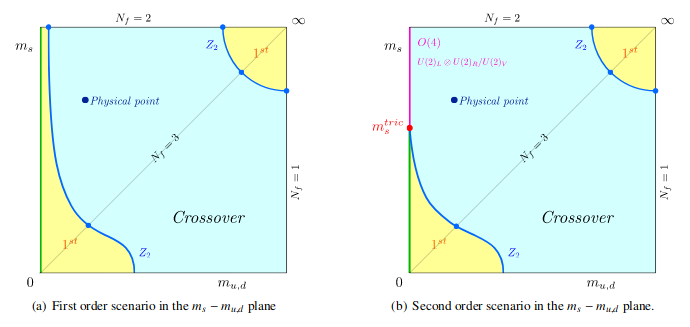
\includegraphics[width=1.0\textwidth]{columbia.png}
%\end{minipage}
%\hfill
%\caption{Two possible scenarios for the Columbia Plot with the up and down quark mass taken to be identical. The ``physical point" is the Standard Model. Plot from \cite{Cuteri:2017zcb}
%}
%\label{fig:columbia}
%\end{figure*}
We now study the nature of the QCD phase transition across the different sectors. Due to the confining nature of QCD, the exact nature of the phase transition is often difficult to ascertain analytically and requires the study of lattice simulations. In the SM, it is known that the phase transition is a crossover and does lead to gravitational wave signals~\cite{Aoki:2006we,Bhattacharya:2014ara}. In the general case with 3 or more colours, the phase transition can be strongly first order in two regimes~\cite{Panero:2009tv,SVETITSKY1982423,Pisarski:1983ms}:
\begin{itemize}
\item Three or more light flavours.
\item No light flavours. 
\end{itemize}
Light means mass small compared to the confinement scale $\Lambda_{QCD}$, but what that means quantitatively is not precisely determined. In the SM, the up and down quarks are light, but the strange is not sufficiently light for an SFOPT.
% The results of these studies on the nature of QCD phase transitions is summarized in the so-called ``Columbia" plot (Fig. \ref{fig:columbia}). As seen in the above figure (and explicitly demonstrated through lattice studies \cite{lattice}), our sector is solidly in the weak-cross over area. In order to observe the strong first order transition required for gravitational wave production, at least some of the additional sectors present must feature quarks in either the heavy quark (pure Yang-Mills) or massless limits.    
%
%In the Yang-Mills limit we see $m_{u,d,s} \rightarrow \infty$. This leads to the presence of a global $Z_3$ centre symmetry that is broken at high temperatures but restored low temperatures. Ultimately, this restoration results in a first order phase transition \cite{SVETITSKY1982423}. On the other end of the spectrum, ``massless" quark theories ($m_q \ll \Lambda_{QCD}$ for all quarks) also contain strong phase transitions due to the breakdown of SU$(N)\,\times$ SU$(N)$ chiral symmetry \cite{Pisarski:1983ms}. Both the Yang-Mills and massless limit arguments can be generalized to SU$(N \geq 3)$: coupling both with the additional restriction that we avoid the conformal window indicates that strong first order phase transitions can occur if we have $n = 0$ (pure Yang-Mills) or $3 \leq n < 4N$ (light quark limit) very light flavours.
For the standard sectors in our setup, the quark masses increase with increasing vev, so for sufficiently large $i$, all the quarks will be heavier than $\Lambda_{QCD}$,\footnote{$\Lambda_{QCD}$ does vary with $i$, but the sensitivity is very weak as we will see below.} and those large $i$ sectors will undergo an SFOPT if they are reheated above the the confinement scale. 
%For $N$naturalness (or other mirror sector models), standard sectors with higher vevs possess more massive quarks; eventually, sectors with large enough vevs push us into the upper-right corner. 
Conversely, exotic sectors with zero vev feature six very light quarks, so \textit{all} the exotic sectors undergo SFOPT at the temperature of QCD confinement. 
We now calculate the QCD confinement scale for each sector following the same procedure as \cite{Cui:2011wk}. First, due to the parameters of each sector being taken to be identical save for the higgs mass squared (thus $v \neq v_i$, where $v$ is the SM vev), we assume that the strong coupling of every sector is identical at some high scale. Using the one-loop running, the $\beta$ function can be solved:
\begin{equation}\label{eqn:QCDrunningi}
\alpha_{s}^i (\mu) = \frac{2\pi}{11-\frac{2n^i_f}{3}}\frac{1}{\ln{\mu/\Lambda^i}},
\end{equation}
where $n_f^i$ is the number of quark flavours with mass less than $\mu/2$ and $\Lambda^i$ is the scale where it would confine if all quarks remain massless. In the SM defined at scales well above all the quark masses, we have $\Lambda_{QCD} = 89 \pm 5$ in $\overline{MS}$~\cite{PhysRevD.98.030001}. 
Because we've set the strong couplings equal at high scales, $\Lambda = \Lambda^i$ for all $i$ at high scales for all sectors. However, since the masses of the quarks in each sector are different, we end up with a unique running of the coupling for each sector. At every quark mass threshold for a given sector, we match the coupling strengths above and below the threshold and determine the new $\Lambda^i$ for the lower scale. For example, at the mass of the top quark, we match a five flavour coupling with the six flavour one:
\begin{equation}
\alpha_s^{i(5)}(2 m^i_t) = \alpha_s^{i(6)}(2 m^i_t) 
\end{equation} 
and thus
\begin{equation}
\Lambda_{(5)}^i = (m_t^{i})^{2/23}(\Lambda_{(6)}^i)^{21/23}.
\end{equation}
Suppressing the $i$'s for notational cleanliness, we can arrive at similar relations at the bottom and charm thresholds
\begin{equation}
\begin{split}
\Lambda_{(4)} = (m_b)^{2/25}(\Lambda_{(5)})^{23/25},
\\
\Lambda_{(3)} = (m_c)^{2/23}(\Lambda_{(4)})^{25/27}.
\end{split}
\end{equation}
These can be combined to show that
\begin{equation}
\Lambda_{(3)} = (m_t m_b m_c)^{2/27}(\Lambda_{(6)})^{21/27}.
\end{equation}
This type of matching procedure can be done as many times as necessary for a given sector. The process terminates when $\Lambda_i$ for a given scale is larger than the next quark mass threshold (i.e running the scale down arrives at the $\Lambda_{QCD}$ phase transition before reaching the next quark mass scale).
In cosmological terms, we can envision a sector's thermal history unfolding, whereas the plasma cools below each quark mass threshold and said quarks are frozen out. At a certain point, the sector arrives at the QCD phase transition and confinement occurs (provided there are light enough quarks to confine) --- if this occurs when $\geq 3$ quarks are at a much lower scale or all quarks have already frozen out, we get the desired phase transition.   
\subsection{Standard Sectors}
As shown in Eq.~(\ref{eqn:vevs}), for standard sectors with increasing index $i$ the vevs of said sectors increase $v_i\propto \sqrt{i}$. This leads to increasingly heavy particle spectra for higher sectors --- eventually leading to sectors that are essentially pure Yang-Mills that feature strong first order phase transitions. This, of course, begs the question: at what index $i$ do said phase transitions begin?
%The actual boundary of region of interest on the Columbia plot is not precisely known and further lattice simulations are required to determine exactly where in parameter space cross-over transitions end and first order transitions begin. In lieu of such studies, we parameterize our ignorance in the form of a ``slop factor" $\kappa$. Assuming the up and down quarks of each sector to be of roughly the same scale, we determine what sector $i$ features $\kappa m_u^i \approx \Lambda_{QCD}$.
Using the methods outlined in the prior section we determine $\Lambda_{QCD}$ to have a relevant value of 
\begin{equation}\label{eqn:lambda2}
\Lambda^i_{(2)} = (m_s^i m_c^i m_b^i m_t^i)^{2/29}(\Lambda^i_{(6)})^{21/29}
\end{equation} 
at the energy scale we're interested in. $\Lambda^i_{(6)}$ is identical for all sectors and is taken to have a standard model value of $\Lambda^{(6)}_{MS} =(89 \pm 6)\, \mev$~\cite{PhysRevD.98.030001}. Rewriting Eq.~(\ref{eqn:lambda2}) in terms of standard model variables, 
\begin{equation}\label{eqn:lambda2adj}
\Lambda^i_{(2)} = (m_s m_c m_b m_t i^2)^{2/29}(\Lambda_{(6)})^{21/29}.
\end{equation}
We take the sector with SFOPT to be the ones when the mass of the up quark, down quark, and QCD phase transition scale are all comparable:
\begin{equation}
m^i_u \sim m_u \sqrt{i} \sim (m_s m_c m_b m_t i^2)^{2/29}(\Lambda_{(6)})^{21/29}.
\end{equation}
This can be solved for $i$:
\begin{equation}\label{eqn:critIndex}
i^c \sim \frac{(m_s m_c m_b m_t)^{4/21}(\Lambda_{(6)})^{2}}{( m_u)^{58/21}} \sim 10^6.
\end{equation}
As we will see in Sec.~\ref{sec:reheat}, in the original $N$naturalness setup~\cite{Arkani-Hamed:2016rle}, the energy dumped into the $i$th sector scales as $i^{-1}$, so there will will not be enough energy in the sectors with $i>i^c$ to see a signature of these phase transitions. 
%This critical index demonstrates that even in the most extreme cases, where first order phase transitions occur with the up quark an order of magnitude less than $\Lambda_{QCD}$, the critical index is still $\sim 1000$. Looking back to the energy density scaling in Eq.~(\ref{eqn:edSS})\textcolor{green}{refer to a particular equation} we see that, within the context of $N$naturalness, the energy density of these sectors is at most $10^{-4}$ \textcolor{green}{why not $10^{-3}$?} that of our sector. As a result, \textcolor{green}{As we will show below?} the gravitational waves generated by the standard large $i$ sectors in $N$naturalness will not generate detectable signatures. 
However, if we move away from the original $N$naturalness reheating mechanism and begin exploring mirror sectors with large vevs and with relative energy densities $\rho_i / \rho_{SM} \sim 10\%$, a possibility allowed by current constraints, we can have sectors with relatively high dark QCD scales that produce detectable gravitational waves. From Eq.~(\ref{eqn:lambda2}) we can determine the confinement scale of an arbitrary mirror sector. If we take Higgs vevs as high as the GUT scale $\sim 10^{16}$ GeV, then we can get confinement scales as high as $\sim 38 \,\gev$.  The signals of this sector and other test cases like it are explored in Sec. \ref{sec:gw}. 
\subsection{Exotic Sectors}
In every exotic sector the fermion masses are exceptionally light: their masses are generated by dimension six operators with the Higgs integrated out as shown in Eq.~(\ref{eqn:exoticFM}), and are therefore all below the confinement scale. The exotic sectors all have identical one-loop running of the QCD gauge coupling, and thus all have approximately the same confinement scale given by $\Lambda_{\rm ex} \sim 90 \,\mathrm{MeV}$. These sectors all have six light fermions, so a strong first order phase transition occurs for all exotic sectors at this temperature. 
The confinement of these sectors directly leads to the production of both baryons and mesons as we have the spontaneous breaking of SU$(6) \,\times$ SU$(6) \rightarrow\,$ SU$(6)$ and thus 35 pseudo-Goldstone bosons (pions). The masses obtained through the phase transition can be approximated through the use of a generalization of the Gell-Mann--Oakes--Renner relation~\cite{Gell-Mann,Schwartz:2013pla},
\begin{equation}\label{eqn:gmor}
m^2_{\pi} = \frac{V^3}{F^2_{\pi}}(m_u + m_d),
\end{equation}
where $V \sim \Lambda_{QCD}$, $F_\pi$ is the pion decay constant. One expects that within a given sector $F_\pi \sim V \sim \Lambda_{QCD}$ \cite{Schwartz:2013pla} and as exotic sectors have $\Lambda_{ex} \sim 90 \,\mev$ while the SM features $\Lambda_{QCD} = (332\pm17)\,\mev$ \cite{PhysRevD.98.030001} we expect at most $\mathcal{O}(1)$ difference in the $\sqrt{\frac{V^3}{F_\pi^2}}$ coefficient relative to the SM value. So, for pions in exotic sector $i$:
\begin{equation}
m_{\pi}^i \sim \sqrt{\frac{m_a^i+m_b^i}{m_u + m_d}} m_{\pi}.
\label{eq:ith_pion_mass}
\end{equation}
Here, $a$ and $b$ denote the component quark flavours. 
\section{Reheating N Sectors}
\label{sec:reheat}
%\begin{figure*}[tb]
%\centering
%\begin{minipage}[c]{\textwidth}
%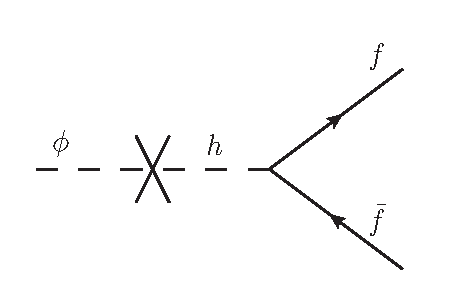
\includegraphics[width=0.4\textwidth]{standardDecay.eps}
%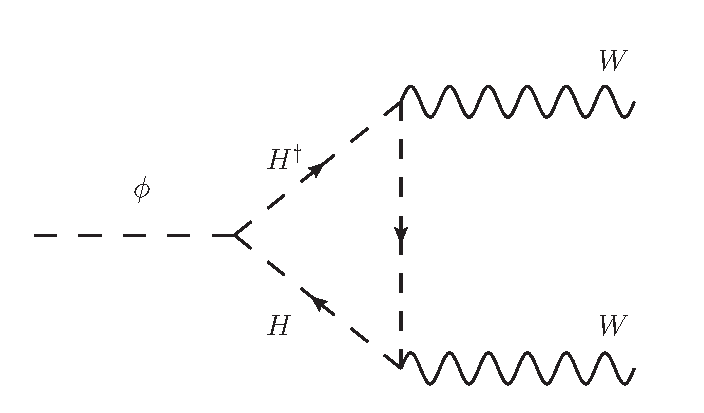
\includegraphics[width=0.4\textwidth]{exoticDecay.eps}
%\end{minipage}
%\hfill
%\caption{Feynman diagrams for primary reheaton decays assuming $m_{\phi} \ll m_H$. The left decay is the primary decay for standard sectors ($\langle H\rangle\neq 0$), with $f$ representing all possible fermions. The right decay occurs in exotic sectors ($\langle H\rangle = 0$).
%}
%\label{fig:reheatonDecays}
%\end{figure*}
A key issue within $N$naturalness is how to predominantly gift energy density to our own sector so as to not be immediately excluded by cosmological constraints, particularly those from number of effective neutrinos ($N_{eff}$). In~\cite{Arkani-Hamed:2016rle} this is done through the introduction of a post-inflationary field called the ``reheaton". After inflation, the reheaton field possess the majority of the energy density of the Universe. Although this field can generically be either bosonic or fermionic, we reduce our scope to a scalar reheaton $\phi$. Our focus is primarily the production of gravitational waves from multiple sectors and a fermion reheaton does not change the scaling of the energy density of the exotic sectors and thus does not affect expected gravitational wave profiles.
In order to maintain the naturalness of our SM sector, the reheaton coupling is taken to be universal to every sector's Higgs. However, a large amount of the Universe's energy density must ultimately be deposited in our own sector for $N$naturalness to avoid instant exclusion. In order to accomplish this the decay width into each sector must drop as $\vert m_H\vert$ grows. If we insist that the reheaton is a gauge singlet that is both the dominant coupling to every sector's Higgs and lighter than the naturalness cutoff $\Lambda_H/\sqrt{N}$ then we construct a model that behaves as desired. 
The appropriate Lagrangian for a scalar reheaton $\phi$ is: 
\begin{equation}\label{eqn:nnLagrangian}
\cL_\phi \supset -a\phi\sum_i\vert H_i\vert^2 - \frac{1}{2}m^2_\phi \phi^2.
\end{equation}
Note that cross-quartic couplings of the form $\kappa\vert H_i\vert^2\vert H_j\vert^2$ that could potentially ruin the spectrum of $N$naturalness are absent, taken to be suppressed by a very small coupling. Effective Lagrangians for the two different types of sectors present in this theory can be obtained by integrating out of the Higgs bosons in every sector:
\begin{equation}\label{eqn:nnEffLag}
\begin{split}
\cL_\phi^{v \neq 0} &\supset C_1 a y_q\frac{v}{m_h^2}\phi q q^c,
\\
\cL_\phi^{v = 0} &\supset C_2 a \frac{g^2}{16\pi^2 m_H^2}\phi W_{\mu\nu}W^{\mu\nu},
\end{split}
\end{equation}
with $C_i$ representing numerical coefficients, $g$ the weak coupling constant, and $W^{\mu\nu}$ the SU$(2)$ field strength tensor.
Immediately from Eq. (\ref{eqn:nnEffLag}), we can see that the matrix element for decays into standard sectors is inversely proportional to that sectors higgs mass, $\cM_{m_H^2 < 0} \sim 1/m_{h_i}$ (since $v\sim m_H$). 
%The Feynman diagram for this process is presented in Fig. \ref{fig:reheatonDecays}. 
The loop decay of $\phi \rightarrow \gamma\gamma$ is always sub-leading and can be neglected. It should be noted that as one goes to sectors with larger and larger vevs, the increasing mass of the fermions ($m_f \sim v_i \sim v_{SM}\sqrt{i}$) eventually leads to situations where the decay to two on-shell bottom or charm quarks is kinematically forbidden, $m_\phi < 2 m_q$. For sectors where this kinematic threshold is passed for charm quarks, the amount of energy in these sectors becomes so small that contributions to cosmological observables can be safely ignored. All in all, we end up with a decay width that scales as $\Gamma_{m_H^2<0} \sim 1/m_h^2$. Since we can expect energy density to be proportional to the decay width, $\frac{\rho_i}{\rho_{SM}} \approx \frac{\Gamma_i}{\Gamma_{SM}}$, this indicates that energy density of standard sectors falls:
\begin{equation}\label{eqn:edSS}
\rho_i \sim r_{s}\frac{\rho_{SM}}{i}
\end{equation} 
with $r_s$ being the ratio of the energy density of the first additional standard sector over the energy density of our sector.
For the exotic sectors, Eq.~(\ref{eqn:nnEffLag}) indicates a matrix element scaling $\cM_{m_H^2>0} \sim 1/m_{H_i}^2$ and is also loop supressed. 
%As the Feynman diagram (Fig.~\ref{fig:reheatonDecays}) shows, the reheaton decays to exotic sectors are loop suppressed, 
This leads to a significantly lower energy density than the standard sectors. Both the decay width and energy density for these sectors scale as: 
\begin{equation}
\Gamma_{m_H^2>0} \sim \rho_i \sim 1/m_H^4 \sim 1/i^2.
\label{eq:reheat_exotic}
\end{equation} 
As a final note, in this setup the reheating temperature of the SM, $T_{RH}$, has an upper bound on the order of the weak scale. If this bound is not observed, the SM Higgs mass would have major thermal corrections --- leading to the branching ratios into other sectors being problematically large~\citep{Arkani-Hamed:2016rle}. Thus we only consider relatively low reheating temperatures $\lesssim 100$ GeV.
Ultimately, after examining the gravitational wave case produced by standard $N$naturalness, we also consider a more general parameterization where sectors are reheated ``randomly" as opposed to in relation to the Higgs mass parameter. This allows us to explore more a broader model space with multiple dark sectors at a huge range of scales. For these models, the reheating mechanism remains undefined and the results of this section are completely irrelevant. 
\section{Constraints}
\label{sec:constraints}
%\begin{figure}
%\centering
%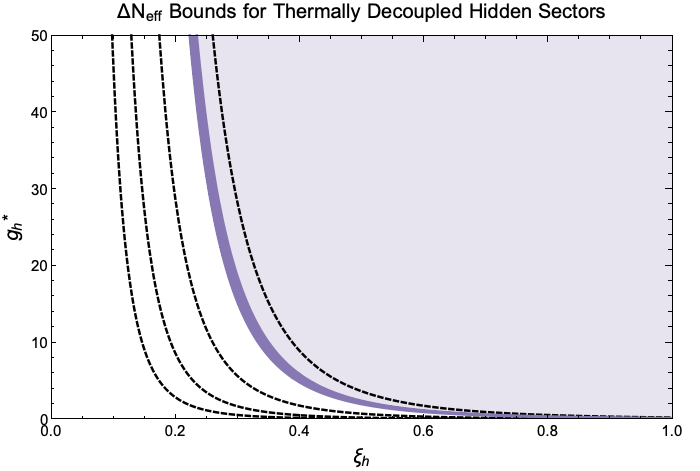
\includegraphics[width=0.45\textwidth]{neff.png}
%\hfill
%\caption{$\Delta N_{eff}$ as a function of relativistic degrees of freedom in a fully decoupled hidden sector ($g_h$) and the temperature ratio of said sector. Contours set $\Delta N_{eff}$ to (0.01, 0.03,  0.1,  0.5) as the dashed lines, from left to right. Most stringent current $N_{eff}$ bounds shade in purple. 
%}
%\label{fig:neff}
%\end{figure}
In general, the multi-hidden sector models explored feature a huge number of (nearly) massless degrees of freedom. Dark photons and dark neutrinos abound in these sectors and, assuming a relatively high reheat temperature, the leptons, quarks, and heavy bosons of these sectors can also be relativistic. In $N$naturalness this feature is realized quite dramatically: each of the $N$ sectors possess relativistic degrees of freedom. The presence of these particles can have two main effects: extra relativistic particles can alter the expansion history of the universe through changes to the energy density or hidden sectors can feature annihilations that reheat the photons or neutrinos of our sector near Big Bang Nucleosynthesis (BBN) and affect the light element abundances. The effective number of neutrino species, $N_{eff}$, is impacted by these contributions and, as such, is the strictest constraint that must be dealt with when studying these type of multi-phase transition models. 
The SM predicts that $N^{SM}_{eff} = 3.046$ \cite{Mangano:2005cc}. This is in good agreement with the $2\sigma$ bounds from studies of the Cosmic Microwave Background (CMB) by Planck combined with baryon acoustic oscillations (BAO) measurements \cite{Aghanim:2018eyx}:
\begin{equation}\label{eqn:neffBounds}
N_{eff} = 2.99^{+0.34}_{-0.33}.
\end{equation}
Various different assumptions about the history of the universe can be made and different data sets can be chosen to obtain slightly different results \cite{Breitbach:2018ddu} --- for the purposes of this exploratory work, wading through this landscape is unnecessary. Additionally, 
\begin{equation}
\frac{(\Delta N^i_{eff})_{CMB}}{(\Delta N^i_{eff})_{BBN}} \geq 1
\end{equation}
for any decoupled hidden sector~\cite{Arkani-Hamed:2016rle}. Because the constraints on $N_{eff}$ are stronger at photon decoupling than at BBN, we can focus purely on the constraints provided by the former.
Future CMB experiments~\cite{Abazajian:2016yjj} will improve the bound from Eq.~(\ref{eqn:neffBounds}) by about an order of magnitude. This could significantly reduce the allowed temperature ratio of any hidden sector, or alternatively could provide evidence for such sectors in a way that is complementary to the gravitational wave signatures described below. 
For fully decoupled sectors that never enter (or reenter) thermal equilibrium with our sector, we obtain additional contributions to $N^{SM}_{eff}$ \cite{Breitbach:2018ddu}
\begin{equation}\label{eqn:DeltaNeff1hs}
\Delta N_{eff} = \frac{4}{7}\left(\frac{11}{4}\right)^{4/3}g_h \xi_h^4.
\end{equation} 
Here, $g_h$ represents the effective number of relativistic degrees of freedom for the hidden sector\footnote{$g_h = N_{\rm boson} + 7 N_{\rm fermion}/8$.}, and we parameterize the hidden sector temperature by~\cite{Breitbach:2018ddu}
\begin{equation}
\xi_h \equiv  \frac{T_{h}}{T_{\gamma}},
\label{eq:xi}
\end{equation}
and these should be evaluated at the time of photon decoupling. 
%
%
%when the hidden sector has a temperature $T_h = \xi_h T_\gamma$. \draftnote{These should be defined at the time of CMB decoupling?} 
%Contours for Eq. (\ref{eqn:DeltaNeff1hs}) at various temperature ratios as well as CMB bounds are plotted in Fig.~\ref{fig:neff}. 
We take this approach and generalize it to include many additional sectors:
\begin{equation}\label{eqn:DeltaNeff}
\Delta N_{eff} = \sum_i \frac{4}{7}\left(\frac{11}{4}\right)^{4/3}g_{i} \xi^4_{i}.
\end{equation} 
For a dark sector with one relativistic degree of freedom, its temperature must be $\sim 0.6\, T_{\rm SM}$ to not be excluded. This sector would have an energy density $\rho \sim 0.036\, \rho_{\rm SM}$. 
%\draftnote{Maybe give what the temperature ratio should be for one standard (or exotic) sector to not be excluded.} 
%As Fig.~\ref{fig:neff} \textcolor{green}{Why is it figure V?} demonstrates, sectors with a temperature ratio above $\xi_h\sim 0.6$ with even a couple of relativistic particles are immediately excluded by CMB constraints. Accordingly, the additional sectors present in this project must be heated to a much smaller fraction of our own sector's temperature. \textcolor{green}{$\xi=0.5$ and $g=2$ is not excluded.}
\subsection{Exotic Sector Contributions}
%The original $N$naturalness paper focused on the (stronger) $N_{eff}$ constraints from the additional standard sectors and ignored the exotic sectors altogether \cite{Arkani-Hamed:2016rle}; in contrast, we take the opposite approach. Since we're more interested in a more general scenario with multiple dark phase transitions, we focus in on whether zero vev sectors can dodge these $N_{eff}$ bounds. 
We begin by computing the constraints on exotic sectors; these are significantly weaker than those for standard sectors~\cite{Arkani-Hamed:2016rle}. 
%At high scales, these sectors feature 106.75 effective degrees of freedom at high energies: 72 from quarks,  12 from charged leptons, 6 from neutrinos, 16 from gluons, 2 from photons, 6 from W bosons (no longitudinal modes due to a no symmetry breaking), 4 from the higgs sector (again, no symmetry breaking leads to 3 additional modes), for a total of 118 degress of freedom. Scaling the fermionic contributions by $7/8$ gives us 106.75 effective relativistic degrees of freedom.  After the higgses freeze out, 4 degrees of freedom are lost; when the QCD phase transition occurs 35 bosonic degrees of freedom are gained while 72 fermionic are lost, leaving 56.75 effective degrees of freedom. 
At the time of photon decoupling ($T_\gamma \sim 0.39 \,\ev$) while the temperature of the exotic sectors is lower still. This means that for sectors with small and moderate $i$, we can use Eqs.~(\ref{eqn:exoticFM}) and~(\ref{eq:ith_pion_mass}) to see that the pions will be non-relativistic  leaving at most $11.25$ effective degrees of freedom per sector from photons and neutrinos.  For very large $i$, the pions can be much lighter, but those sectors also have very little energy in them in the standard reheating scenario. 
%Since all additional sectors are colder than our own, by the time photon decoupling occurs ($T_\gamma \sim 0.39 \,\ev$), the pions of all of these sectors will, in accordance with Eq.~(\ref{eqn:gmor}), have a much higher mass than the sector temperature and thus will have frozen out long before --- leaving at most $11.25$ effective degrees of freedom per sector from photons and neutrinos. \draftnote{Pions are not decoupled at BBN time, does this in any way affect the analysis?}
Coupling the number of effective degrees of freedom per sector with the energy density scaling of $\sim 1/m_H^4$ as in Eq.~(\ref{eq:reheat_exotic}) means that the zero vev sectors have small temperature ratios. Assuming a reheating temperature of $100$ GeV and a completely uniform distribution of sectors, the temperature of the first exotic sector is slightly more than $6\%$ of our sector at reheating. Applying Eq.~(\ref{eqn:DeltaNeff}) to this particular situation gives us:
\begin{equation}
\Delta N_{eff} = \sum_i \frac{4}{7}\left(\frac{11}{4}\right)^{4/3}g_{i} \left(\frac{(T_{RH_{E1}}/T_{RH})}{i^{1/2}}\right)^4 \sim 10^{-4},
\end{equation}     
with $T_{RH_{E1}}/T_{RH}$ being the ratio of the reheat temperatures of the 1st exotic sector and our own sector ($0.06$ in standard $N$naturalness with $r = 1$).  This sum is dominated by $i=1$, the sector with the lowest Higgs mass (and thus the most energy density) gives us a contribution of $\mathcal{O} (10^{-4})$ to $\Delta N_{eff}$. Evolving the sectors thermal histories forward in time to the recombination era gives us a slightly larger value, but still of order $\mathcal{O}(10^{-4})$, well under current CMB bounds. 
It should be noted that modifying the exotic sectors' structure (e.g. adjusting the exotic sectors to have a lower higgs mass squared or clustering multiple hidden sectors close to the first exotic one) leads to a $\Delta N_{eff}$ contribution that is larger than the base $N$naturalness case. This increase is typically not excluded by current bounds, indicating a large degree of liberty in the structure and number of exotic hidden sectors.
\subsection{Generalized Reheating Scenarios}
The generalization of possible reheating mechanisms mentioned in section~\ref{sec:reheat} --- where the reheating mechanism no longer depends on the higgs' mass parameter of a given sector --- opens up a wide range of hidden sectors for study. Specifically, this allows mirror sectors with large Higgs vevs to be reheated to significant energy densities and thus produce gravitational waves with enough power to be detected. Crucially, despite this analysis being limited to mirror sectors with large Higgs masses, this analysis pertains to any strong, confining phase transition at high scales.
Since $N_{eff}$ constraints remain our strongest cosmological bounds for massive standard sectors, our starting point for exploring the limits of high transition temperatures is Eq.~(\ref{eqn:DeltaNeff}). Assuming heavy, standard sectors (with the only relativistic particles being photons and neutrinos) we can saturate the bounds of Eq.~(\ref{eqn:neffBounds}) and solve for the maximum temperature allowed for any number of sectors:
\begin{equation}\label{eqn:energyDensityAllowed}
\begin{split}
T_i &\sim 0.38 \,T_{SM} \,\,\,\,\, \mathrm{1}\,\, \mathrm{hidden}\,\, \mathrm{sector},
\\
T_i &\sim 0.25 \,T_{SM} \,\,\,\,\, \mathrm{5} \,\,\mathrm{hidden}\,\, \mathrm{sectors},
\\
T_i &\sim 0.21 \,T_{SM} \,\,\,\,\, \mathrm{10} \,\,\mathrm{hidden}\,\, \mathrm{sectors},
\\
T_i &\sim 0.12 \,T_{SM} \,\,\,\,\, \mathrm{100} \,\,\mathrm{hidden}\,\, \mathrm{sectors},
\end{split}
\end{equation}
where all the hidden sectors have the same temperature as one another.
Using these restrictions, we can examine the behaviour of standard sectors with a much larger vev than our own. In terms of the $N$naturalness framework, this means we can get an SFOPT for QCD if we look at sectors with $i$ greater than the cirtical index of Eq.~(\ref{eqn:critIndex}) where all the quark masses are above the QCD confinement scale. 
 %of looking at various different sectors above the critical index, as mentioned in Sec.~\ref{sec:dQCD}. The signals for both the maximal case ($10^{16}$ limit) and several other high transition temperatures (involving sectors $i > 10^{10}$) scenarios are shown in Sec.~\ref{sec:gw}. \textcolor{yellow}{This assumes that only photons and neutrinos are relativistic? Yes.}
\section{Gravitational Wave Signals}
\label{sec:gw}
%Sectors other than the SM can be reheated through multifield inflationary theories, Reheaton models, etc. In these models, the SM will receive the majority of the energy density while the remaining energy density will be distributed, in a model dependent way, to the various hidden sectors. If there does not exist a portal between the sectors, they will remain decoupled and evolve independently. When looking at multiple thermally decoupled hidden sectors it is convenient to define the temperature ratio [cite cold,dark,noisy]
%\begin{equation}
%\xi_i \equiv  \frac{T_{i}}{T_{\gamma}}
%\end{equation}
%Where $T_{i}$ is the temperature of the $i^{th}$ hidden sector, and $T_{\gamma}$ the temperature of the standard model (assuming radiation domination).
We now turn to the gravitational wave signatures of our setup. At high temperatures, each of the hidden sectors has QCD in the quark/gluon phase, but at temperatures around $\Lambda_{\rm QCD,i}$, the $i^{\mathrm{th}}$ sector undergoes a phase transition into the hadronic phase that we computed for the different sectors in Sec.~\ref{sec:dQCD}. As discussed in that section, this phase transition will be strongly first order (SFOPT) for certain numbers of light quarks, which will generate gravitational waves. This differs from QCD in the SM sector, as the PT is a crossover and not first order~\cite{Fodor:2001pe}. 
%Right after reheating, the temperatures of the respective sectors are high leading to restoration of a given sector's symmetry.  An example being the SM's $SU(3) \times SU(2) \times U(1)$ symmetry being restored as the scalar potential's vev becomes global minimum. As the sectors cool down their scalar potentials may change, producing a new global vev at which the symmetry will break by an induced phase transition. Depending on the characteristics of the symmetry breaking, the phase transition may be strongly first ordered (SFOPT).  
A SFOPT proceeds through bubble nucleation, where bubbles of the hadronic phase form in the vacuum of the quark phase. These bubbles will expand, eventually colliding and merging until the entire sector is within the new phase.  These bubbles are described by the following Euclidean action~\cite{Linde:1981zj}
%
\begin{equation}\label{eqn:EuclideanAction}
S_{E}(T) = \frac{1}{T}\int d^3x \bigg[\frac{1}{2}(\nabla\phi)^2 + V(\phi,T)  \bigg],
\end{equation}
where the time component has been integrated out due to nucleation occuring not in vaccum but in a finite temperature plasma. $\phi$ is the symmetry breaking scalar field with a non-zero vev. In the case of the chiral phase transition, the scalar field breaking the SU$(N_f)_{R}$ $ \times$ SU$(N_f)_{L}$ chiral symmetry is the effective quark condensate $\phi_{i} \sim \langle q\bar{q} \rangle_{i}$ of the respective sector. We leave the thermalized potential $V(\phi, T)$ general. As previously stated, an exact QCD potential at the time of the chiral phase transition is not well understood outside of lattice results. In~\cite{Bai:2018dxf} chiral effective Lagrangian was used to calculate a low energy thermalized potential for confining SU$(N)$. 


The amount of energy density dumped into the individual sectors dictates the energy budget for the PT and hence for the gravitational waves. Assuming that the SM sector is radiation dominated, a quantity that characterizes the strength of the PT is the ratio of the latent heat of the phase transition, $\epsilon$, to the energy density of radiation, at the time of nucleation~\citep{Espinosa:2010hh} ,
\begin{equation}
\alpha     \equiv  \frac{\epsilon}{g_{*} \pi^2 (T^{nuc}_{\gamma})^4/30},
\label{eq:alpha}
\end{equation}
with $\epsilon$ being calculable from the scalar potential. Assuming that there is a negligible amount of energy being dumped back into the SM, which would cause significant reheating of $\rho_{\gamma}$,  the latent heat, $\epsilon$ should correspond to the energy density of the hidden sector going through the PT. The parameter $g_{*}$ in the denominator of Eq.~(\ref{eq:alpha}) is the number of relativistic degrees of freedom at the time of the phase transition, with contributions from species in both the visible and dark sectors. It has weak temperature dependence in a single sector, but when dealing with multiple hidden sectors, $g_{*}$ gains contributions from all $N$ sector's relativistic degrees of freedom, weighted by their respective temperature ratios (energy densities)
\begin{equation}\label{eqn:RelaDOF}
g_{*} = g_{*,\gamma} + \sum_{i} g_{*,i} (\xi_{i})^4,
\end{equation}
with $\xi$ being the temperature ratio defined in Eq.~(\ref{eq:xi}). The bounds from effective number of neutrinos~\citep{Aghanim:2018eyx} mean that $\xi_i \lesssim 1$ for all $i$, so $g_{*} \approx g_{*,\gamma}$. In the case of dark QCD-like chiral  phase transitions, the temperature of the phase transition is on the the order of the symmetry breaking scale of the respective sector, $T_{h}^{i} \sim \mathcal{O}(\Lambda_{QCD,i})$. The work of~\citep{Bai:2018dxf} calculated $\alpha$ with an effective chiral Lagrangian have found various upper bounds. We take the optimistic scenario where the numerator is bounded above by the symmetry breaking scale
%
\begin{equation}\label{eqn:alpha2}
\alpha_i \approx \xi_i^{4} \approx \bigg( \frac{\Lambda_{QCD,i}}{T_{\gamma}^{nuc}}\bigg)^4,
\end{equation}
%
where $T_{\gamma}^{nuc}$ is the temperature of the SM photon bath at the time of the phase transition.

Another important parameter to characterize the phase transition is its inverse timescale, $\beta$~\citep{Caprini:2015zlo}. The inverse timescale can be calculated using the action in Eq.~(\ref{eqn:EuclideanAction}), 
\begin{equation}
\beta  \equiv \frac{dS_{E}(T)}{dt}\bigg|_{t = t_{nuc}}.
\end{equation}
The ratio of $\beta$ and the Hubble constant, at the time of nucleation, $H$ controls the strength of the GW signal,
\begin{equation}\label{eqn:BH}
\frac{\beta}{H} = T^{nuc}_h \frac{dS_{E}(T)}{dT}\bigg|_{T = T^{nuc}_h}.
\end{equation}
Due to the lack of a general analytic QCD potential, it is not possible to use Eq.~(\ref{eqn:BH}) to calculate $\beta/H$. There are dimensional arguments~\cite{Hogan:1984hx,Hogan:1986qda} which predict $\beta/H \sim 4 \textrm{Log}(M_{p}/ \Lambda_{QCD,i})$, although these arguments are riddled with assumptions on the potential. In more recent work, some authors~\citep{Helmboldt:2019pan,Bai:2018dxf} have attempted to estimate it using first-order chiral effective theories and the Polyakov-Nambu-Jona-Lasinio (PNJL) models. These studies claim a large range of values and thus a consensus has not yet been reached.  Under these circumstances, we take the optimistic case in which $\beta/H$ is of order $\mathcal{O}(10)$.
\subsection{Production of Gravitational Waves}
\label{sec:signals}
Gravitational waves are produced with contributions from different components of the SFOPT's evolution.  It is commonplace to parameterize the spectral energy density in gravitational waves by~\citep{PhysRevD.75.043507} 
\begin{equation}
\Omega_{\textrm{GW}} (f) \equiv \frac{1}{ \rho_{c}} \frac{d \rho_{\textrm{GW}}(f) }{d \textrm{\,log}(f)} , 
\end{equation}
where $\rho_{c} = 3H^2/(8 \pi G)$ is the critical energy density. The three leading order contributions to the GW power spectrum are as follows:
\begin{itemize}
\item \textbf{Scalar field contributions $\Omega_{\phi}$}: Caused by collisions of the bubble walls, the solutions being completely dependent on the scalar field configuration. With efficiency factor $\kappa_{\phi} = 1 - \alpha_{\infty}/\alpha$~\citep{PhysRevD.45.4514, Huber_2008}. 
\item \textbf{Sound wave contributions $\Omega_{v}$}: Sound waves within the plasma after bubble collision will produce $\beta/H$ enhanced gravitational waves. With efficiency factor $\kappa_{v} \propto \alpha_{\infty}/\alpha$~\citep{PhysRevLett.112.041301}.
\item \textbf{Magnetohydrodynamical contributions $\Omega_{B}$}: Turbulence within the plasma, left over from the sound wave propagation, will produce gravitational waves. With efficiency factor $\kappa_{
turb} \approx 0.1 \kappa_{v} $~\citep{PhysRevD.74.063521}.
\end{itemize}
Where $\alpha_{\infty}$ denotes the dividing line between the runaway regime  $(\alpha >\alpha_{\infty})$ and the non-runaway regime $(\alpha <\alpha_{\infty})$. Explicitly \cite{Breitbach:2018ddu, Caprini:2015zlo, Espinosa:2010hh}, 
\begin{equation}\label{eqn:critPTstrength}
\alpha_{\infty} = \frac{(T^{nuc}_h)^2}{\rho_R}\left[\sum_{bosons} n_i\frac{\Delta m^2_i}{24} + \sum_{fermions} n_i\frac{\Delta m_i^2}{48}\right],
\end{equation} 
for particles with $n_i$ degrees of freedom that obtain mass through the phase transition. 
Generalized heavy standard sectors feature no baryons due to all quarks being above their respective QCD scales and, as such, produce runaway bubbles similar to the exotic sectors in standard $N$naturalness \footnote {It should also be noted that although free quarks cease to exist post phase transition in these exotic sectors their masses are so light that they do not contribute relevant amounts to $\alpha_{\infty}$.}. 
The total gravitational wave signal is a linear combination of the three contributions:
\begin{equation}
h^2\Omega_{\textrm{GW}} \approx h^2\Omega_{\phi} + h^2\Omega_{v} + h^2\Omega_{turb} .
\end{equation}
In essence, this is a linear combination of the individual spectral shapes weighted by a power of their efficiency factors $\kappa^q$. 
Ultimately, calculating the critical phase transition strength for each sector using Eq.~(\ref{eqn:critPTstrength}) indicates that every sector has a phase transition in the runaway regime. Thus, all exotic sectors have strong first order phase transitions that lead to runaway bubble walls ($\alpha >\alpha_{\infty}$). In this case, the efficiency factors for the sound wave and MHD contributions are small and the GWs produced are dominantly from bubble collisions, $h^2\Omega_{\textrm{GW}} \approx h^2\Omega_{\phi}$. Quantities that are calculated at the time of nucleation are denoted with an asterisk (i.e $h^2\Omega_{\textrm{GW}}^*$), which are evolved to relate to their values at the time of observation. The form of the GW energy density at the time of nucleation is given by~\citep{Breitbach:2018ddu},
\begin{equation}
h^2\Omega_{\textrm{GW}}^* = 7.7\times 10^{-2} \bigg( \frac{\kappa_{\phi} \alpha}{1 + \alpha} \bigg)^2 \bigg( \frac{H}{\beta} \bigg)^2  S(f)
\end{equation}
Where we have assumed an optimistic bubble wall velocity of $v \sim 1$ for runaway bubbles. $S(f)$ is the spectral shape function for the signal and a parametric from has been found through numerical simulations~\cite{Huber_2008} of bubble wall collisions.
\begin{equation}\label{eqn::spectralshape}
S(f) = \frac{3.8 \,(f/f_p)^{2.8}}{1 + 2.8\,(f/f_p)^{3.8}}
\end{equation}
The peak frequency, $f_{p}$ is a function of the temperature of the SM at the time of nucleation.  The various hidden sectors can phase transition at different scales and therefore temperatures, causing a shift in the GW spectrum's peak frequency given by~\cite{Huber_2008},
%
\begin{equation}\label{eqn:peakFrequency}
f_{p} = 3.8 \times 10^{-8} \, \textrm{Hz}\, \bigg( \frac{\beta}{H}\bigg)\bigg(\frac{T_{\gamma}}{100 \, \textrm{GeV}}\bigg)\bigg(\frac{g_{*}}{100}\bigg)^{\frac{1}{6}},
\end{equation}
%
where $g_*$  is calculated using Eq.~(\ref{eqn:RelaDOF}) , although, due to the lack of substantial reheating into the hidden sectors, the SM contribution is dominant. 
Now that the framework has been laid out for the creation of GW from a single SFOPT, we generalize to multiple sectors going under independent, coherent SFOPT. In the models presented in this paper, we consider a subset of N-hidden sectors that phase transition at a SM temperature of $T_{\gamma}^{i}$. As the GWs propagate in free space, the energy density and frequency spectrum, at the time of production $\Omega_{\textrm{GW}}^{*}(f)$, will redshift to today's value $\Omega_{\textrm{GW}}^{0}(f) = \mathcal{A}\, \Omega_{\textrm{GW}}^{*}((a_{0}/a) f) $. The Redshifting factor, $\mathcal{A}$, accounts for the redshifting of both $\rho_{\textrm{GW}} $ and $\rho_{c}$~\cite{Breitbach:2018ddu,PhysRevD.49.2837}, given by:
\begin{equation}\label{eqn::redshifting}
\mathcal{A} \equiv \bigg( \frac{a}{a_{0}} \bigg)^4 \bigg( \frac{H}{H_{0}}\bigg)^2,
\end{equation}
where $a$ ($a_{0}$)  and $H$ ($H_{0}$) are the scale factor and Hubble constant at the time of nucleation (observation), respectively. Assuming that the sectors are completely decoupled before and after their respective SFOPT, the total GW signal that would be measured today is given by the coherent sum,
\begin{equation}
\Omega_{\textrm{GW}} =  \sum_{i}^{N} \mathcal{A}^{i}\, \Omega_{\textrm{GW}}^{i,*}((a_{0}/a)_{i} f) .
\end{equation}
We assume that the parameters of the SFOPT do not differ between sectors: the relativistic degrees of freedom, phase transition rate, and the dark QCD scale, are all similar. This makes the redshifting factor $\mathcal{A}^i$ independent of sector number.
\begin{figure}[h!]
\centering
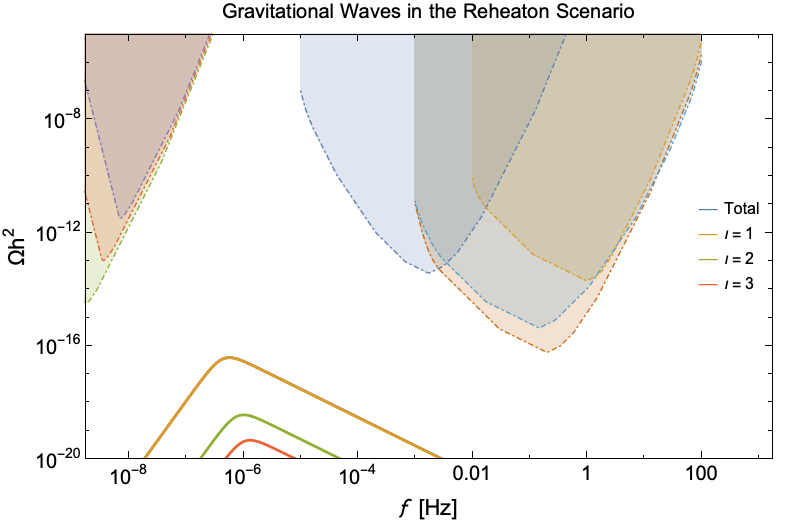
\includegraphics[scale=.3]{Nnatral.png} 
\caption{ Gravitational wave power spectrum for standard $N$naturalness using the scalar reheaton model of section~\ref{sec:reheat}. All contributions are assumed to be purely from bubble collisions $\Omega_{\phi}$, with $\beta/H  = 10$.  The shaded curves are the power law noise curves~\cite{PhysRevD.88.124032} calculated from expected sensitivity curves for space-based interferometers and pulsar timing arrays as described in Section~\ref{sec:detection}; Lisa ( blue), DECIGO (light blue), BBO (red), SKA 5-year (purple), SKA 10-year (orange), SKA 20-year (green).}
\label{fig::Nnatural}
\end{figure}
Applying this to the standard reheating scenario of $N$natrualness, introduced in~\ref{sec:reheat}, we get GW signals as seen in figure~(\ref{fig::Nnatural}). Plotted are the individual contributions to the signal from each phase transitioned sector, as well as the coherent sum of all sectors. Future GW interferometers and pulsar timing array sensitivity curves are shown in comparison to the signal. The sensitivity curves are interpreted as the region of possible detection if intersected with the GW signal, more detail in the construction of these curves is given in Section~\ref{sec:detection}. Notice that the total signal is dominated by the first sectors contribution. This is caused by the quartic temperature ratio suppression in Eq.~(\ref{eq:alpha}) and the large temperature gaps between adjacent sectors. Such a suppression leads to standard $N$natrualness evading future detector thresholds by a few orders of magnitude in units of energy density. 

This is not the case if we consider the more generalized reheating scenarios of Sec.~\ref{sec:constraints}. Once the restriction that sectors with small higgs' masses are preferentially reheated has been lifted, we can explore a much more vast landscape of hidden sectors than are allowed in the vanilla case. Here, we construct several different scenarios that are both detectable and demonstrate a variety of gravitational wave profiles. Specifically, we explore scenarios that lead to a deviation in the peak behaviour of the total GW signal (the convolution of stochastic GW from individual SFOPT) from a standard power law signal.

It should be noted that the key phenomenological constraint on all of these models is $\Delta N_{eff}$, giving us a maximum allowed temperature ratio (when compared to the SM) for each reheated hidden sector: Eq.~(\ref{eqn:energyDensityAllowed}) shows the maximum temperature ratios for specific numbers of additional hidden sectors. Due to the rather harsh scaling of the GW strength, $\alpha$, with temperature ratio (Eq.~(\ref{eqn:alpha2})), we take the optimistic approach of keeping the temperature ratio as high as possible for all of the hidden sectors.

In all our examined cases, we focus on heavy standard sectors --- pure Yang-Mills sectors with much heavier particles (specifically quarks) and, as shown in Sec.~\ref{sec:dQCD}, the SFOPT these entail. The reason for this arises from Eq.~(\ref{eqn:peakFrequency}): every exotic sector features a phase transition that occurs at $\Lambda_{ex} \sim 90$ MeV. If we maximize the allowed temperature ratio, this gives us a (SM) photon temperature, $T_{\gamma}$, that places our signal directly into the void between the detection region of pulsar timing arrays and space-based interferometers (see Sec.~\ref{sec:detection}). The location of the peak can be changed by dropping the temperature ratio, but the adjustment required to end up with a signal with an appropriate peak frequency makes the overall signal too weak to detect. In accordance with Sec.~\ref{sec:dQCD}, standard sectors can have much higher temperature phase transitions. As such, maintaining the maximum allowed temperature ratio between the hidden sector(s) and the SM gives a much larger photon temperature and a proportionally larger peak frequency; ultimately allowing for detection by space-based interferometers.

There are four scenarios that we examine here:
\begin{itemize}
\item \textbf{Maximized signal:} A single additional heavy hidden sector which saturates all current experimental bounds. The SM photon bath temperature at the time of the hidden sector PT is $87$ GeV. In the $N$naturalness framework this is equivalent to reheating a standard sector with $i\sim 10^{16}$ up to the maximum allowed temperature ratio.
\item \textbf{Large split scenario:} A scenario where two additional hidden sectors have been reheated --- these sectors have higgs vevs that are split by a factor of $\sqrt{10^3} = (v_{h1})/(v_{h2})$. This results in a difference in the scale of the SFOPTs leading to the SM photon bath temperature changing a large amount during the time between the PTs. This, in turn, leads to a large separation in the peak frequency of their gravitational wave signals.  In the $N$naturalness framework this is equivalent to reheating two standard sectors, one with $i\sim 10^{12}$ and another with $i\sim 10^{15}$ up to the maximum allowed temperature ratio.
\item \textbf{Medium split scenario:} Similar to the previous case: these sectors have higgs vevs that are split by a factor of $\sqrt{10}= (v_{h1})/(v_{h2})$, resulting in a much smaller difference in the peak frequency of their gravitational wave signals. In the $N$naturalness framework this is equivalent to reheating two standard sectors, one with $i\sim 10^{12}$ and another with $i\sim 10^{13}$ up to the maximum allowed temperature ratio.
\item \textbf{Five sector scenario:} Five sectors are reheated to the maximum allowed temperature ratio, each with vevs that are $\sqrt{3} \sim (v_{hi})/(v_{h(i+1)})$ larger than the previous sector.
\end{itemize}
The GW results of these cases are presented in figure~(\ref{fig:Haa}). In all cases, the summed GW signal is detectable by one or more proposed interferometers. When relaxing the assumptions on $\beta/H$, the scenarios in figure~(\ref{fig:Haa}) are still detectable for values ranging between $\mathcal{O}(1)$ and $\mathcal{O}(100)$ The frequency dependence in Eq.~(\ref{eqn::spectralshape}) takes the form of $f/f_{p}$, this causes a cancellation between the redshifting factors. As multiple sectors phase transition at different times, and therefore temperatures, the peaks will shift relative to each other, purely from the linear temperature dependence of the peak frequency $f_{p} \sim T_{\gamma}$.  This is seen in figure~(\ref{fig:Haa}), where the spectrum peaks are shifted causing a peak broadening of the convoluted spectrum. The broadening can be substantial if the hidden sectors transition between a large gap of time. Assuming that the amplitudes of individual contributions are comparable, a temperature gap limit exists at which two or more individual peaks could be resolved.

\begin{figure*}[tb]
\centering
\begin{minipage}[c]{\textwidth}
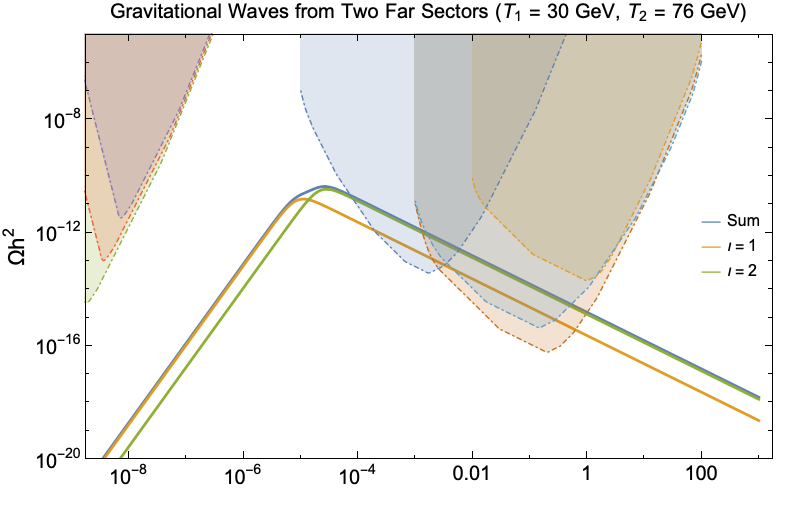
\includegraphics[width=.45\textwidth]{TwoFar.png} 
\hfill
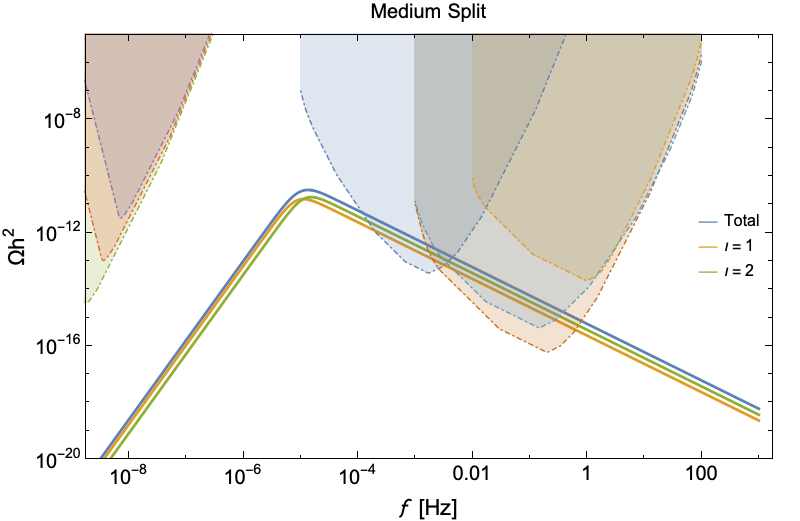
\includegraphics[width=.45\textwidth]{TwoMed.png} 
\hfill
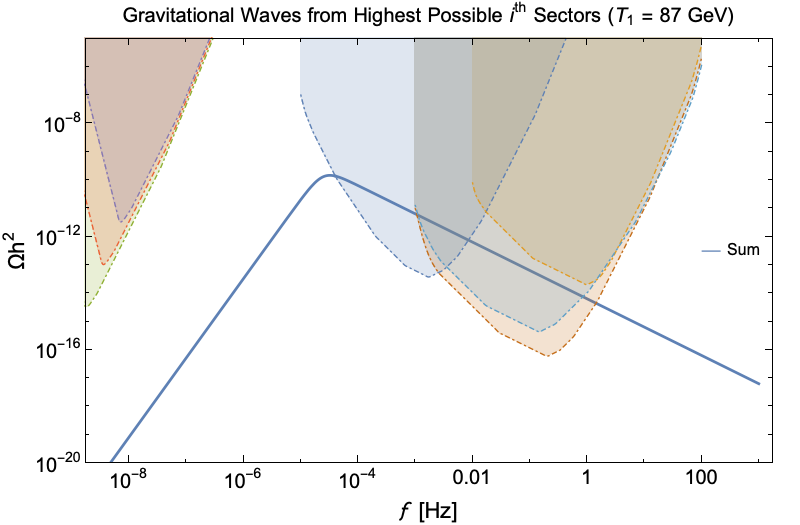
\includegraphics[width=.45\textwidth ]{highest.png}
\hfill
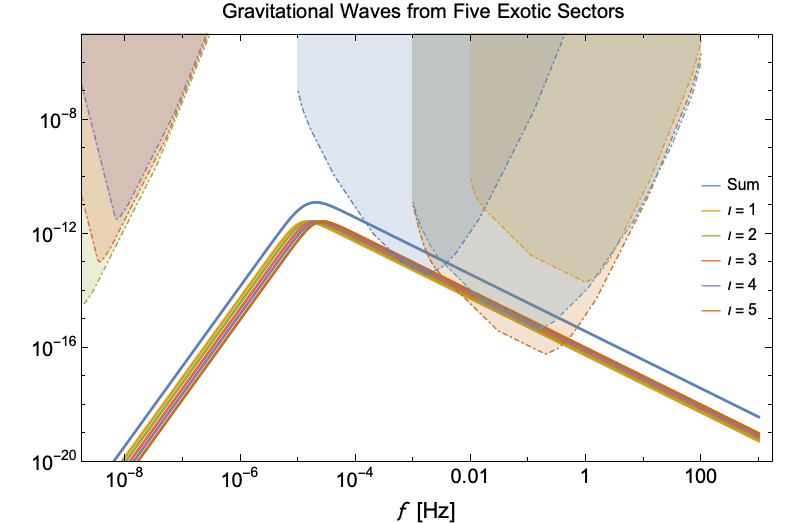
\includegraphics[width=.45\textwidth]{energydensity.png} 
\end{minipage}
\hfill
\caption{ Gravitational wave power spectrum for various models. The top row consists of two models with only two hidden sectors undergoing SFOPT at differing temperatures. The bottom left (right) are examples of exotic sectors, discussed in section V, with sectors reheated at $T \sim 0.25\,T_{SM}$ ($T \sim 0.17\,T_{SM}$ ). All contributions are assumed to be purely from bubble collisions $\Omega_{\phi}$, with $\beta/H  = 10$.  The shaded curves are the power law noise curves~\cite{PhysRevD.88.124032} calculated from expected sensitivity curves for space-based interferometers and pulsar timing arrays; Lisa ( blue), DECIO (light blue), BBO (red), SKA 5-year (purple), SKA 10-year (orange), SKA 20-year (green)   }
\label{fig:Haa}
\end{figure*}
\subsection{Detection of Stochastic Graviational Waves}
\label{sec:detection}
A unpolarized stocastic gravitational wave background could be detectable if the the signal-to-noise ratio (SNR) is above some threshold value, $\rho > \rho_{th}$, dictated by the capabilities of future interferometers and pulsar timing arrarys (PTA). These interferometers/PTAs quote their experimental sensistivies in terms of spectral noise curves, $S_{\textrm{eff}}(f)$, which can be translated into units of energy density through $h^2 \Omega_{\textrm{eff}}(f) = \frac{2\pi^2}{3H^2}f^3 S_{\textrm{eff}}(f)$. If the experiment uses a single (multiple) detector, the auto-correlated (cross-correlated) SNR is used in comparing to the threshold value $\rho_{th}$. The auto-correlated and cross-correlated SNR are explictely given as~\cite{PhysRevD.59.102001},
\begin{equation}\label{eqn::SNR}
\begin{split}
\rho^2 =  T \int_{f_{\textrm{min}}}^{f_{\textrm{max}}}\textrm{d}f \bigg( \frac{h^2 \Omega_{\textrm{GW}}(f)}{h^2 \Omega_{\textrm{eff}}(f)} \bigg)^2 \;\;\;\;\;\; \textrm{(auto-correlated)},
\\
\rho^2 = 2 T \int_{f_{\textrm{min}}}^{f_{\textrm{max}}}\textrm{d}f \bigg( \frac{h^2 \Omega_{\textrm{GW}}(f)}{h^2 \Omega_{\textrm{eff}}(f)} \bigg)^2 \;\;\;\: \textrm{(cross-correlated)},
\end{split}
\end{equation}
where $T$ is the exposure time of the experiment. The integration covers the entire broadband range of frequencies $(f_{\textrm{min}}, f_{\textrm{max}})$. LISA~\citep{Audley:2017drz} and B-DEICIGO~\citep{10.1093/ptep/pty078} are proposed to be single detector interferometers, where as BBO~\citep{PhysRevD.72.083005} and DEICIGO~\citep{Sato_2017} would be built from an array of multiple interferometers.
GW signals produced from an early cosmological phase transition would be seen as a stocastic background. Assuming that the GW follows a power law background in frequency, it is commonplace to quote the power law integrated (PLI) sensistivity curves~\cite{PhysRevD.88.124032}. The PSI curves are constructed using information from the power law form of the signal,
\begin{equation}
h^2 \Omega_{\textrm{GW}}(f) = h^2 \Omega_{\beta}  \bigg(\frac{f}{f_{\textrm{ref}}}\bigg)^{\beta},
\end{equation}
where $\beta$ is the spectral index of the power law, and $f_{\textrm{ref}}$ is an arbitrary reference frequency which has no effect on the PLI sensetivities. 
The method of calculating the PLI curves involves plotting $h^2 \Omega_{\textrm{GW}}(f) $, using Eq.~(\ref{eqn:RelaDOF}), for various spectral indices $\beta \in (-8,-7,-6, ... , 6, 7, 8)$ and for some fixed threshold value of $\rho_{th}$. Each curve will lay tangent to the PSI curve, more formally,
\begin{equation}
h^2 \Omega_{\textrm{PLI}} = \max\limits_{\beta}\bigg[ h^2 \Omega_{\beta}\bigg(\frac{f}{f_{\textrm{ref}}}\bigg)^{\beta}  \bigg].
\end{equation}
The spectral noise curves used to create the PSI curves shown in figures~(\ref{fig::Nnatural}) and ~(\ref{fig:Haa}) where taken from~\citep{Robson_2019,PhysRevD.83.084036,doi:10.1142/S0218271813410137,10.1093/ptep/pty078, Breitbach:2018ddu} for the interferometers, and ~\citep{Breitbach:2018ddu, Janssen:2014dka} for the SKA pulsar timing array. We have assumed an observation time of $T = 4 $ years for the interferometers and $T= 5, 10, 20 $  years for the various stages of SKA. In the case of the PTA experiments, the sensitivity curves are dependent on how frequently the pulsar's timing residuals, $\delta t$, are measured. When using Eq.~(\ref{eqn::SNR}) to construct the PSI curves for SKA, the upper integration bound is inversely proportional to pulsar's timing residual, $f_{min} = 1/\delta t$. In this work, it is assumed that $\delta t = 14$ days, but this may underestimate the capabilities of SKA as well as the cadences of the pulsar populations. If the timing residuals are lowered the maximum frequency reach of SKA increases, and the corresponding PSI curves in Figs.~(\ref{fig::Nnatural}) $\&$ ~(\ref{fig:Haa}) are shifted to the right.
\section{Conclusion}
\label{sec:conclusion}

As detection capabilities increase, gravitational wave signals continue to grow in importance as phenomenological signatures that can offer us a unique glimpse into the universe as it was in the early epochs. The space-based interferometers planned for the next generation of GW experiments will be sensitive enough to begin searching for signals of the cataclysmic disruption of space-time due to SFOPT. As we inch closer to these measurements becoming available, it becomes important to develop ways to analyze and understand this data.

Here, we examined several scenarios (including $N$naturalness) that involve multiple hidden sectors and calculated the GW profiles present. Our GW projections demonstrate that although vanilla $N$naturalness is not projected to be detectable in the near future, more generalized scenarios with multiple hidden sector SFOPTs are in an observable region and will begin to be probed by next generation space experiments. Both cases feature important parts of their GW signals in the void between frequencies detectable by pulsar timing arrays and space-based interferometers --- providing theoretical impetus for new experiments capable of probing this region of frequency space. 

Further, our results provide a framework for understanding and using GW signals in two opposite ways: first as a unique signal for specific theories featuring multiple SFOPTs and also as a way to explain signals that deviate from a standard power law spectrum. 

In the former case, this demonstrates the power of GW signals to probe deep into the unknown arena of complex hidden sectors. Whether a model predicts of the presence of 1, 5, or more hidden sectors, any SFOPT can potentially contribute a GW signal and the sum of these signals can create a unique GW background; ultimately providing another means to test and constrain theories.   

Shifting to the latter scenario, should a stochastic GW background be detected, deviations from a standard power law curve would indicate a more complicated hidden sector. Individual SFOPT are understood to create GW that are assumed to follow an approximate power law. The multiple transitions that occur in the models outlined here create signals that do not respect this trend: although the individual GW do obey approximate power laws, their sum does not --- leading to a unique signal indicating so-called dark complexity. Explicitly, a broadening or distortion of the signal around the peak frequency could point to a multi-SFOPT scenario and gently guide us in the direction of multiple hidden sectors. 

%Questions, of course, still abound: how can the %estimations of $\alpha$ and $\beta/H$ be improved? 

%%%%%%%%%%%%%%%%%%%%%%%%%
%%%%%%%%%%%%%%%%%%%%%%%%%
%%%%%%%%%%%%%%%%%%%%%%%%%
%%%%%%%%%%%%%%%%%%%%%%%%%
%%%%%%%%%%%%%%%%%%%%%%%%%
\appendix
%%%%%%%%%%%%%%%%%%%%%%%%%%%%%
\bibliographystyle{apsrev4-1}
\bibliography{refs}
\end{document}






